Essa capítulo tem como por propósito apresentar o modelo, sua utilização para um dado estudo de caso e sua implementação 
em Prolog (linguagem de programação com viés na Lógica Matemática). O modelo foi construindo usando Teoria de Conjuntos
e Lógica de Predicado.

Os conjuntos são usados para representar um dado conceito. Os elementos de um conjunto representam os objetos atrelados ao 
conceito. Por exemplo, supondo que uma lógica de Carros venda os seguintes veículos; \textit{Jetta}, \textit{Gol}, \textit{Uno}.
Nesta situação, o conceito de carro é represdentado pelo conjunto $C$ e os módelos são elementos do mesmo. Portanto, numa linguagem
matemática formal tem-se a seguinte situação $C = \{Jetta,Gol,Uno\}$. 

Dentro do conceito matemático, uma relação é uma correspondencia entre elementos de conjuntos não vazio, sendo dada por
$R \subseteq  A \times B = \{(a,b)| a \in A \wedge b \in B \}$. A Lógica de Predicados foi usada para representar essas
relações. Para representação das regras foi feito uso das relações de inferência $\rightarrow$ "Se ..., então ...".  

O \textit{UML} também é uma ferramenta que foi usada para criar representações do modelo. O propósito disto consiste nos
seguintes aspectos; apresentar perspectiva global do modelo, definir melhor os critérios existenciais (agregação, composição),
tornar o processo de apresentação mais didático e aproxima-lo de mecanismos de implementação (ex. linguagens de programação). 

A figura \ref{module} apresenta a estrutura de módulos (a fim de evitar poluição visual, as relações serão apresentadas
em outra figura). 

\begin{figure}[H]
  \centering
  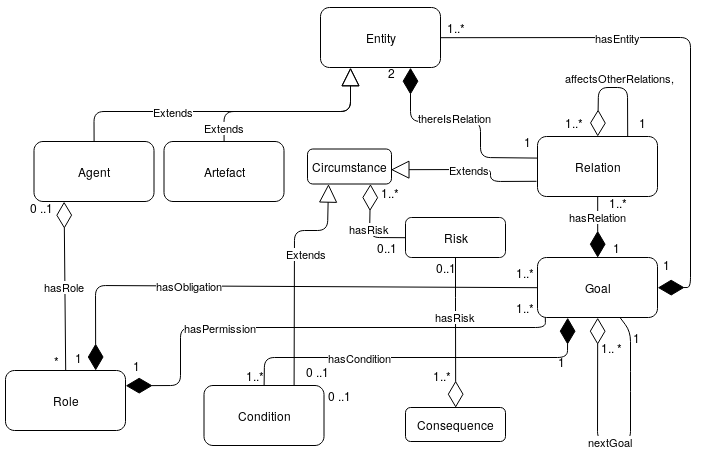
\includegraphics[width=1\linewidth]{figure/Class.png} 
  \caption{A estrutura geral das classes do modelo}
  \label{module}
\end{figure}

Assim sendo, assumindo que existe $\Omega_{Model}$ (um conjunto global onde todos os outros conjuntos do modelo estão 
contidos nele), os módulos são representados da seguinte maneira; 

\begin{equation} 
    \Omega_{Model} = \{ M_{Risk}, M_{Task}, M_{Entity}, M_{Environment}\}
\end{equation}
\label{modules}
